\documentclass[11pt]{article}

\usepackage[letterpaper, margin=1in]{geometry}

\usepackage[spanish]{babel}
\usepackage[utf8]{inputenc}
\usepackage{multirow}
\usepackage{tabularx}
\usepackage{longtable}



%Figuras
\usepackage{graphicx, subfigure}
\usepackage[]{tikz}
\usepackage{pbox}

%Matemática
\usepackage{amsmath}
\usepackage{amssymb}

%Símbolos mate extra (alfabetos, etc.)
\usepackage{mathrsfs}


%Algoritmos
\usepackage{float}
\usepackage{algorithm}
\usepackage{algorithmicx}
\usepackage{algpseudocode}
\usepackage{listings}


\usepackage{color}
\usepackage{hyperref}

\usepackage{mdframed}
\usepackage{tcolorbox}
\usepackage{multicol}
\usepackage{booktabs}
\usepackage{tabulary}
\definecolor{darkblue}{rgb}{0 , 0.054 , 0.196}



\title{Reporte de laboratorio 4}
\author{Laura Rincón Riveros - B55863\\Esteban Vargas Vargas - B16998\\ Grupo 3}

\begin{document}

\maketitle
\hrule
\hrule
\tableofcontents
\hspace{5mm}
\hrule
\hrule

%%%%%%%%%%%%%%%%%%%%%%%%%%%%%%%%%%%%
\section{Introducción}
%%%%%%%%%%%%%%%%%%%%%%%%%%%%%%%%%%%%

En el presente laboratorio se realizó una revisión bibliográfica para poder sintetizar los conceptos de problemas con complejidad NP, NP-duros y NP-completos. Asimimso se realizó una búsqueda sobre problemas clásicos de las complejidades mencionadas.

En la segunda parte del laboratorio se analizó un código fuente proporcionado por el profesor y se obtuvo su función de tiempo de ejecución y su complejidad \textit{O}; adicionalmente se elaboraron gráficas para representar con facilidad los datos.


\newpage
%%%%%%%%%%%%%%%%%%%%%%%%%%%%%%%%%%%%
\section{Desarrollo}

\subsection{Conceptos de complejidad de problemas}

\subsubsection{Problemas NP}
Un problema \textit{NP} se define como un problema que se puede resolver mediante un algoritmo con una función de tiempo de ejecución no polinomial en una máquina determinista. 
\subsubsection{Problemas NP-duros}
Si se tiene un conjunto de problemas \textit{NP}, un problema es \textit{NP-duro} si la duración de todos esos problemas \textit{NP} se puede 
transformar mediante un factor polinomial en la duración del problema \textit{NP-duro}.

\subsubsection{Problemas NP-completos}

Un problema es NP-completo si se puede reducir con una función polinomial en una función polinomial también; y además la verificación de su instancia también es polinomial. 

\newpage 
%%%%%%%%%%%%%%%%%%%%%%
\subsection{Problemas clásicos}
\subsubsection{Problemas NP}
\begin{itemize}
\item El problema de factorizar números en una multiplicación de números primos: cuando la cifra es grande el problema es intratable. 
\item El problema de isomorfismo de grafos: consiste en la determinación de si dos grafos con el mismo número de vértices y aristas son isomorfos o no. No se conoce si es resoluble en tiempo polinómico o si es \textit{NP-completo}.
\end{itemize}
\subsubsection{Problemas NP-duros}
\begin{itemize}
\item Problema de la suma de subconjuntos: dado un conjunto de enteros, la pregunta es si existe algún subconjunto en él cuya suma sea cero. (Problema también es \textit{NP-completo}).
\item El problema del agente viajero: dado un viajero y un conjunto de ciudades, el problema es encontrar cuál es la distancia más corta posible en la que el viajero puede visitar todas y volver a su punto de origen. 
\end{itemize}
\subsubsection{Problemas NP-completos}
\begin{itemize}
\item El problema SAT de la satisfactibilidad de la lógica proposicional. (Fue el primer problema demostrado ser NP-completo, por S.A. Cook en 1971).
\item El problema de \textit{Clique}: es un problema de decisión de si un grafo contiene un \textit{clique} de al menos un tamaño k. (Un clique se le dice a un subgrafo con todos los vértices conectados entre ellos).
\end{itemize}
%%%%%%%%%%%%%%%%%%%%%%
\newpage 
\subsection{Programa TicTacToe}
\subsubsection{Explicación}
El programa en \textbf{ttt.src} contiene el algoritmo de un juego de TicTacToe para dos jugadores. El cuál se basa en una matriz cuadrada, cada jugador ingresa una posición y el programa verifica si el valor asignado para ese jugador está en una columna, fila o digonal completa. Si se cumple lo anterior se determina el ganador o se continúa hasta que alguno gane.
\subsubsection{Función de tiempo de ejecución}

\begin{figure}[H]
\centering
\subfigure[Función move]{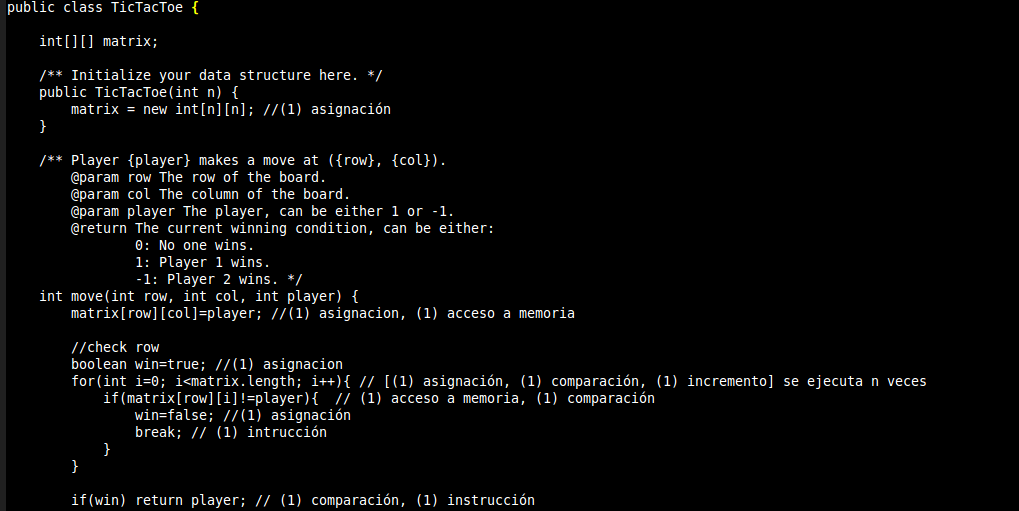
\includegraphics[height=12cm, width=\textwidth]{img/move.png}}
\subfigure[Main]{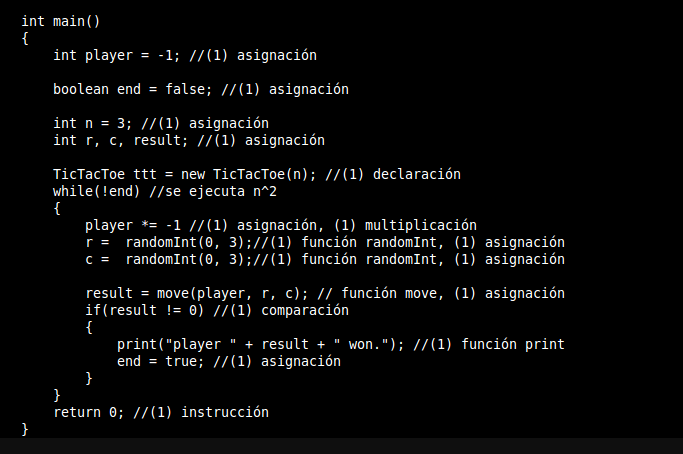
\includegraphics[height=9.5cm, width=\textwidth]{img/main.png}}
\caption{Conteo para obtener función del tiempo}
\label{fig:cont}
\end{figure}
 
\footnote{Revisar el archivo \textbf{ttt.src} comentado y contado} Se procedió a contar cada intrucctivo para cuantificar el tiempo de ejecución de todo el programa. 
 
 Por lo que, se puede observar en la Figura \ref{fig:cont}.a se encuentra la declaración de las variables y la función de move. Para el caso de la función del progama, las verificaciones como se repiten se obtiene lo siguiente:
 
 \begin{equation}
T_{1}(n)= 1 + 1 + 4*(1 + [(1 + 1 + 1)n*(1+ 1 + 1 + 1)]) + 1 + 1 + 1 + 1 = 48n+10
\end{equation}
 
 Si agregamos los intrucctivos del main y la inicialización de las variables a (1), de la Figura \ref{fig:cont}.b:
 
 \begin{equation}
T(n)= 1 + 1 + 1 + 1 + 1 + 1 + [n^{2}*(1 + 1 + 1 + 1 + 1 + 1 + 48n + 10 + 1 + 1 + 1 + 1)] + 1 =  48n^{3} + 20n^{2} + 7
\end{equation}
 
 La función de tiempo dada por (2) pertenece a todo el programa. Y se puede observar en la Figura \ref{fig:graf}, la segunda gráfica.
 
 \begin{figure}[H]
\centering
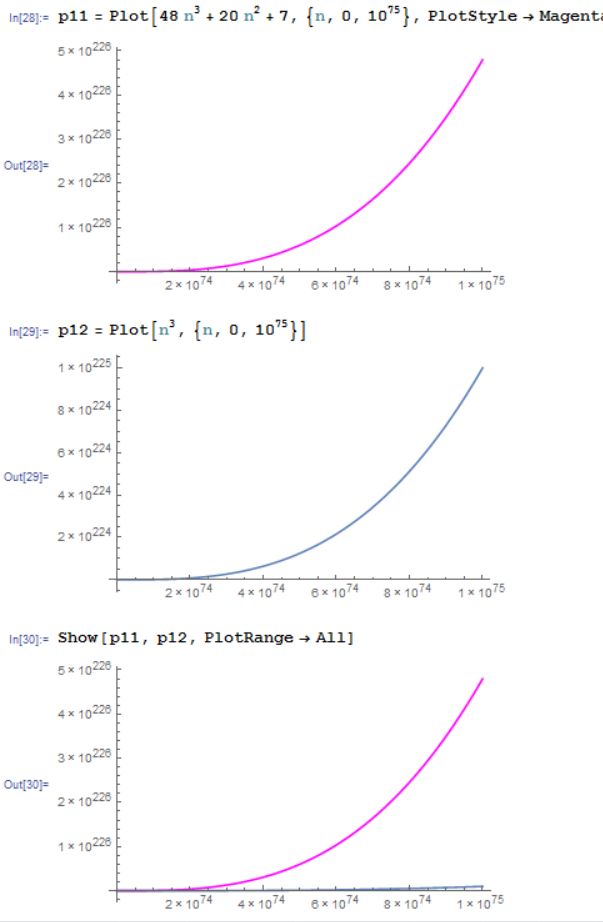
\includegraphics[height=18cm, width=17cm]{img/Grafica1.png}
\caption{Conteo para obtener función del tiempo}
\label{fig:graf}
\end{figure}
 

\newpage
\subsubsection{Función de complejidad O}

Si se simplifica la función de tiempo, se puede obtiene la función de complejidad $O(n^3)$, que se puede representar en la Figura \ref{fig:graf}, la primera gráfica.
También se puede ver que O(n) acota inferiormente a T(n), en la tercera gráfica de la Figura \ref{fig:graf}


%%%%%%%%%%%%%%%%%%
%%%%%%%%%%%%%%%%%%%%%%


\newpage
%%%%%%%%%%%%%%%%%%%%%%
 
\newpage
%%%%%%%%%%%%%%%%%%%%%%%%%%%%%%%%
\section{Conclusiones}
%%%%%%%%%%%%%%%%%%%%%%%%%%%%%%%%
\begin{itemize}
\item Se describieron y explicaron los conceptos de complejidades NP, NP-dura y NP-completos.
\item Se estudiaron los problemas clásicos de las distintas complejidades NP.
\item Se obtuvo la función de tiempo y comlejidad del programa \textbf{ttt.src}
\item Se graficaron las funciones de tiempo y complejidad del programa proporcionado.
\end{itemize}

\begin{thebibliography}{15}

\bibitem{1}Pérez, M.Sancho,F. (2003). \textit{Máquinas moleculares basadas en ADN}. Sevilla, España: Secretariado de Publicaciones de la Universidad de Sevilla. 

\bibitem{2} \textit{Complejidad-ProblemasNP-Completos}. Algoritmos y estructuras de datos III. Recuperado de $https://www.dc.uba.ar/materias/aed3/2014/2c/teorica/handout_compl.pdf$. 

\end{thebibliography}


\end{document}
